\textbf{Linear correlations}\newline
\noindent
The linear regression between simple features, number of pain pixels or active pain regions, and outputs, pain duration or pain intensity, resulted in the plots shown in fig. \ref{fig:correlations}. The $R^2$-values support the nonlinearity, shown in the plots, where correlation fig. \ref{fig:1} resulted in a $R^2 = 0.018$, fig. \ref{fig:2} resulted in $R^2 = 0.008$, fig. \ref{fig:3} resulted in $R^2 = 0.011$ and fig. \ref{fig:4} resulted in $R^2 =  0.011$. \\

\begin{figure*} [t!]
\begin{tcolorbox}[colframe=black!30!black, colback=white]
\hfill
\begin{subfigure}[r]{0.5\textwidth}
    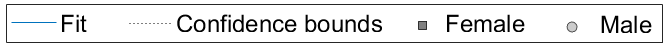
\includegraphics[width=\textwidth]{Figures/legend}
  \end{subfigure}
  \vskip\baselineskip
  \hspace{-5mm}
  \begin{subfigure}[b]{0.51\textwidth}
    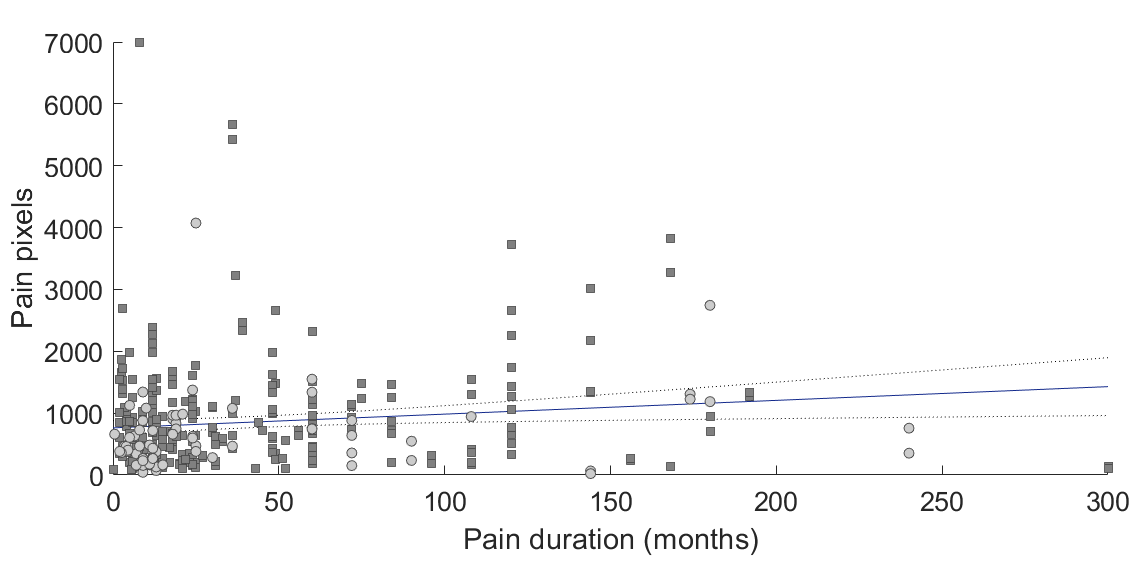
\includegraphics[width=\textwidth]{Figures/durapixel}
    \caption{ }
    \label{fig:1}
  \end{subfigure}
  \hfill
    \hspace{2mm}
  \begin{subfigure}[b]{0.51\textwidth}
    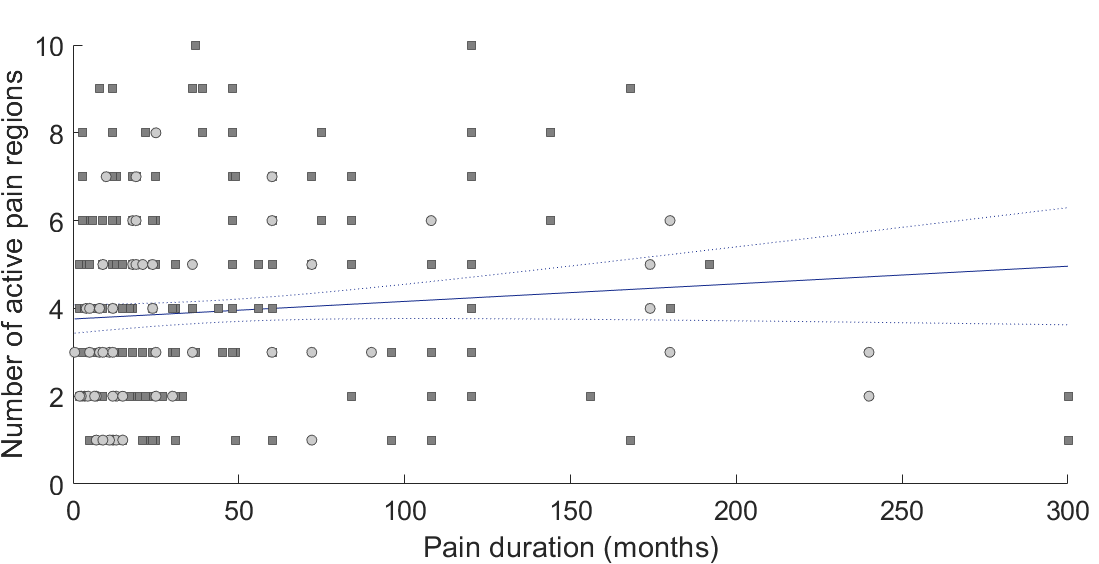
\includegraphics[width=\textwidth]{Figures/duraregion}
       \caption{ }
    \label{fig:2}
  \end{subfigure}
    \vskip\baselineskip
    \hspace{-5mm}
  \begin{subfigure}[b]{0.51\textwidth}
    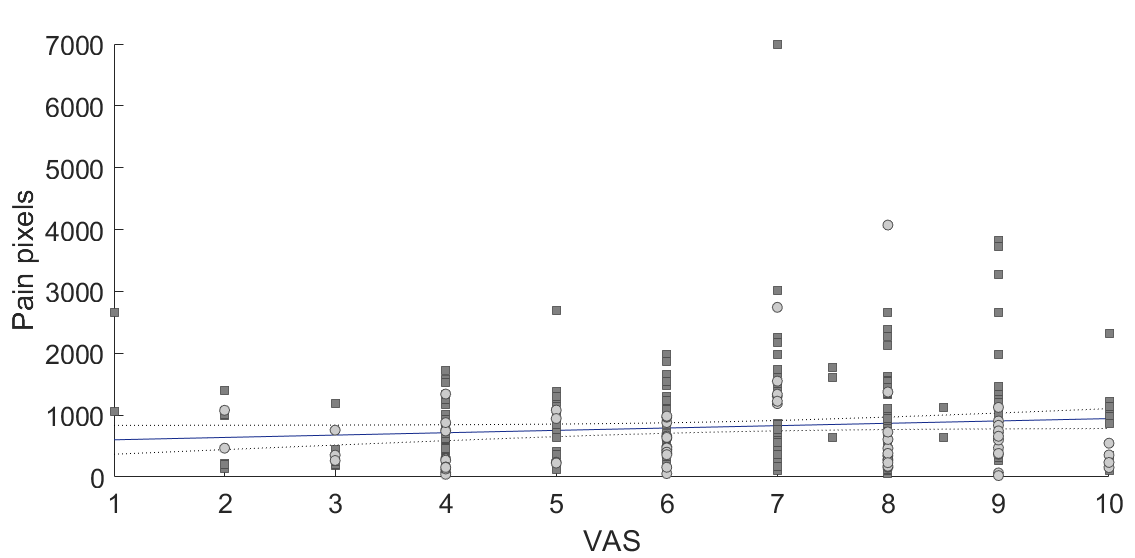
\includegraphics[width=\textwidth]{Figures/vaspixel}
    \caption{}
    \label{fig:3}
  \end{subfigure}
  \hfill
  \hspace{2mm}
  \begin{subfigure}[b]{0.51\textwidth}
    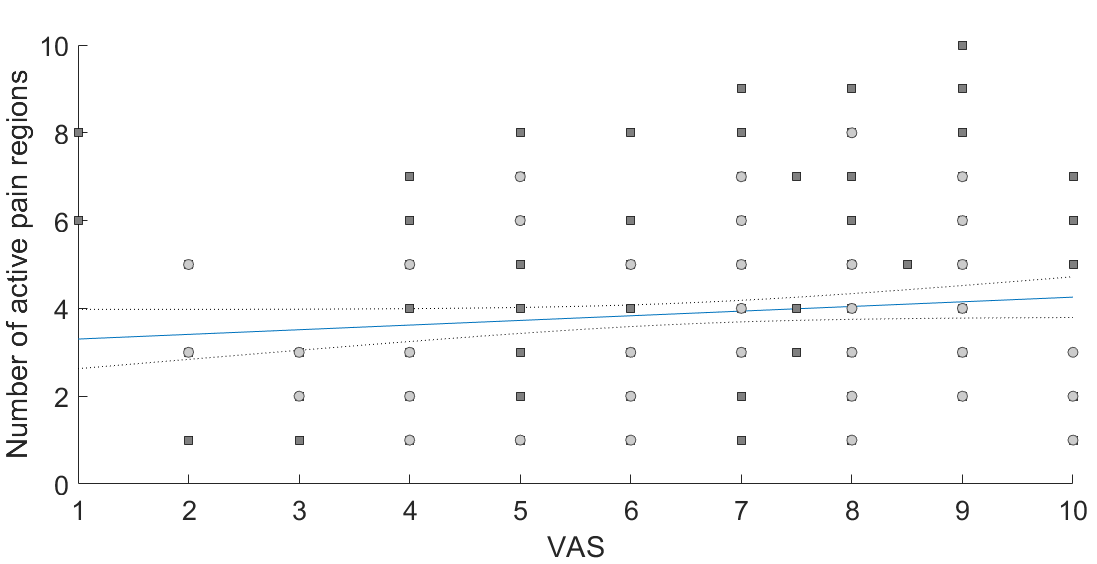
\includegraphics[width=\textwidth]{Figures/vasregion}
       \caption{ }
    \label{fig:4}
  \end{subfigure}  
  \caption{Linear correlations of pain pixels and pain duration (a), active pain regions and pain duration (b), pain pixels and pain intensity indicated in VAS (c), and active pain regions and pain intensity indicated in VAS (d).}
  \label{fig:correlations}
\end{tcolorbox}
\end{figure*}

\newpage

\noindent
\textbf{Classification according to outputs}\newline
\noindent
tyfuihoj \\


\noindent
\textbf{Classification of pain maps}\newline
\noindent
yubi







Results on generalization performance when using 10-fold cross validation, after final optimization for morphology-, region- and combined representation are shown in tab. \ref{tab:performance}. This is done for pain duration and pain intensity classifications to which an average accuracy, sensitivity, and specificity are calculated along with it’s corresponding standard deviations. 


\begin{table*}[b]
\centering
\begin{tabular}{@{}llll@{}}
\toprule
\multicolumn{4}{c}{\hspace{2.3cm} Avg. accuracy (\%) \hspace{1cm} Avg. sensitivity (\%) \hspace{1cm} Avg. specificity (\%) \hspace{1cm}                }                                                                                                                                                                         \\ \midrule
\multicolumn{4}{c}{Morphology-representation} \\ \midrule
Pain duration  & \hspace{0.7cm}\begin{tabular}[c]{@{}l@{}}59.51\% \\ ($\pm 11.20\%$)\vspace{0.3cm}\end{tabular} & \hspace{2cm} \begin{tabular}[c]{@{}l@{}}62.16\%\\ ($\pm 21.59\%$) \vspace{0.3cm}\end{tabular} & \hspace{2cm} \begin{tabular}[c]{@{}l@{}} 62.20\%\\ ($\pm 18.13\%$) \vspace{0.3cm}\end{tabular} \\ %\midrule
Pain intensity & \hspace{0.6cm} \begin{tabular}[c]{@{}l@{}}65.04\%\\ ($\pm 10.83\%$) \end{tabular}  & \hspace{2.1cm}\begin{tabular}[c]{@{}l@{}}48.23\%\\ ($\pm 0.28\%$) \end{tabular}  & \hspace{2cm} \begin{tabular}[c]{@{}l@{}}71.02\%\\ ($\pm 0.12\%$) \end{tabular}   \\ \midrule
\multicolumn{4}{c}{Location-representation}                                                                                                                                                                             \\ \midrule
Pain duration  & \hspace{0.6cm} \begin{tabular}[c]{@{}l@{}}54.56\%\\ ($\pm 12.81\%$)\vspace{0.3cm}\end{tabular}  & \hspace{2cm} \begin{tabular}[c]{@{}l@{}}50.68\%\\ ($\pm 0.15\%$)\vspace{0.3cm}\end{tabular}  & \hspace{2cm} \begin{tabular}[c]{@{}l@{}}59.55\%\\ ($\pm 0.15\%$) \vspace{0.3cm}\end{tabular}  \\ %\midrule 
Pain intensity & \hspace{0.6cm} \begin{tabular}[c]{@{}l@{}}63.33\%\\ ($\pm 1.67\%$) \end{tabular}   & \hspace{2cm} \begin{tabular}[c]{@{}l@{}}0.00\%\\ ($\pm 0.00\%$) \end{tabular}   & \hspace{2cm} \begin{tabular}[c]{@{}l@{}}63.33\%\\ ($\pm 0.02\%$) \end{tabular}  \\ \midrule
\multicolumn{4}{c}{Combined-representation}                                                                                                                                                              \\ \midrule
Pain duration  & \hspace{0.6cm} \begin{tabular}[c]{@{}l@{}}55.49\% \\ ($\pm 9.55\%$) \vspace{0.3cm}\end{tabular}                                                                   & \hspace{2cm} \begin{tabular}[c]{@{}l@{}}55.23\%\\ ($\pm 0.15\%$) \vspace{0.3cm}\end{tabular}                                                                & \hspace{2cm} \begin{tabular}[c]{@{}l@{}}56.99\%\\ ($\pm 0.12\%$)\vspace{0.3cm}\end{tabular}                                                                                                                                \\% \midrule
Pain intensity & \hspace{0.6cm} \begin{tabular}[c]{@{}l@{}}65.14\% \\ ($\pm 12.87\%$) \end{tabular}
& \hspace{2cm} \begin{tabular}[c]{@{}l@{}} 37.50\%\\ ($\pm 0.35\%$) \end{tabular}                                                               
& \hspace{2cm} \begin{tabular}[c]{@{}l@{}} 67.34\%\\ ($\pm 0.15\%$)\end{tabular}                                                               
 \\ \bottomrule
\end{tabular}
\caption{Generalization performance of the three models, which use the morphology-, location- and combined-representation.}
\label{tab:performance}
\end{table*}